\documentclass[tikz,border=10pt]{standalone}
\usepackage{tikz}

\newcommand{\drawgrid}[4]{
    \foreach \x in {#1,...,#2} {
        \foreach \y in {#3,...,#4} {
            \fill[fill=gray!50, rounded corners=2pt] 
                (\x+0.1, \y+0.1) 
                rectangle ++(0.8, 0.8);
        }
    }
}

\begin{document}

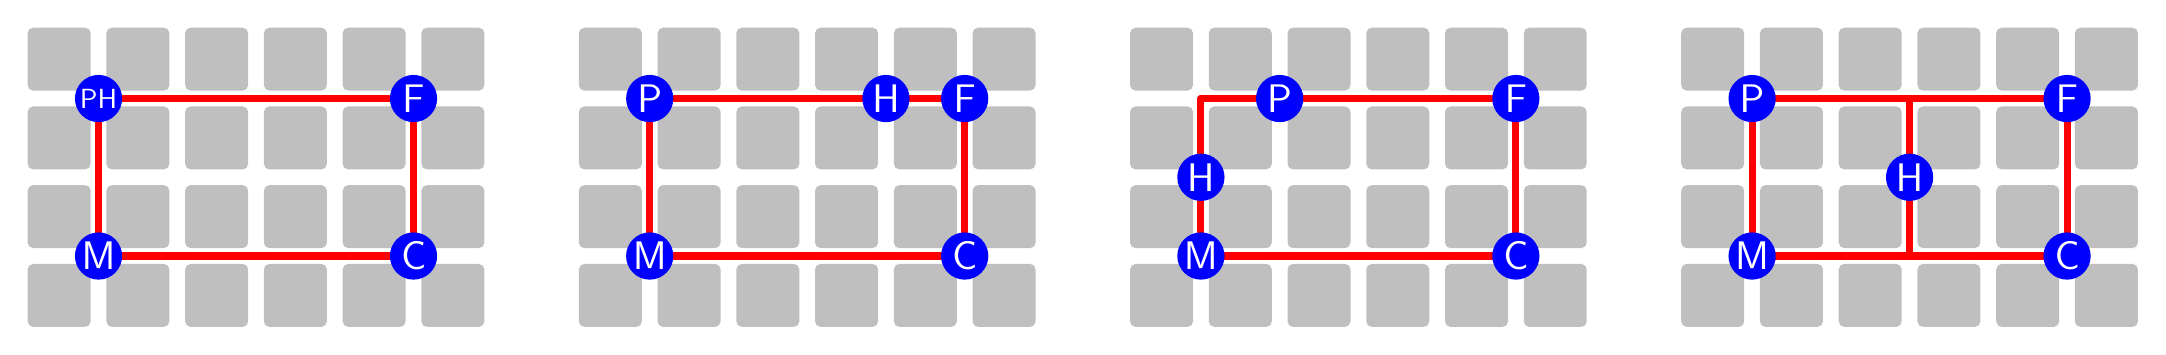
\begin{tikzpicture}[yscale=-1]

\drawgrid{0}{5}{0}{3}
\drawgrid{7}{12}{0}{3}
\drawgrid{14}{19}{0}{3}
\drawgrid{21}{26}{0}{3}


% Highlighted red lines
\draw[red, line width=0.9mm, line cap=round] (1, 1) -- (5, 1);
\draw[red, line width=0.9mm, line cap=round] (1, 3) -- (5, 3);
\draw[red, line width=0.9mm, line cap=round] (1, 1) -- (1, 3);
\draw[red, line width=0.9mm, line cap=round] (5, 1) -- (5, 3);

% Labeled circles with text
\fill[blue] (5, 3) circle (0.3) node[white] {\Large{\textsf{C}}};
\fill[blue] (1, 1) circle (0.3) node[white] {{\textsf{PH}}};
\fill[blue] (5, 1) circle (0.3) node[white] {\Large{\textsf{F}}};
\fill[blue] (1, 3) circle (0.3) node[white] {\Large{\textsf{M}}};


% Highlighted red lines
\draw[red, line width=0.9mm, line cap=round] (8, 1) -- (12, 1);
\draw[red, line width=0.9mm, line cap=round] (8, 3) -- (12, 3);
\draw[red, line width=0.9mm, line cap=round] (8, 1) -- (8, 3);
\draw[red, line width=0.9mm, line cap=round] (12, 1) -- (12, 3);

% Labeled circles with text
\fill[blue] (12, 3) circle (0.3) node[white] {\Large{\textsf{C}}};
\fill[blue] (8, 1) circle (0.3) node[white] {\Large{\textsf{P}}};
\fill[blue] (11, 1) circle (0.3) node[white] {\Large{\textsf{H}}};
\fill[blue] (12, 1) circle (0.3) node[white] {\Large{\textsf{F}}};
\fill[blue] (8, 3) circle (0.3) node[white] {\Large{\textsf{M}}};


% Highlighted red lines
\draw[red, line width=0.9mm, line cap=round] (15, 1) -- (19, 1);
\draw[red, line width=0.9mm, line cap=round] (15, 3) -- (19, 3);
\draw[red, line width=0.9mm, line cap=round] (15, 1) -- (15, 3);
\draw[red, line width=0.9mm, line cap=round] (19, 1) -- (19, 3);

% Labeled circles with text
\fill[blue] (19, 3) circle (0.3) node[white] {\Large{\textsf{C}}};
\fill[blue] (16, 1) circle (0.3) node[white] {\Large{\textsf{P}}};
\fill[blue] (15, 2) circle (0.3) node[white] {\Large{\textsf{H}}};
\fill[blue] (19, 1) circle (0.3) node[white] {\Large{\textsf{F}}};
\fill[blue] (15, 3) circle (0.3) node[white] {\Large{\textsf{M}}};


% Highlighted red lines
\draw[red, line width=0.9mm, line cap=round] (22, 1) -- (26, 1);
\draw[red, line width=0.9mm, line cap=round] (22, 3) -- (26, 3);
\draw[red, line width=0.9mm, line cap=round] (22, 1) -- (22, 3);
\draw[red, line width=0.9mm, line cap=round] (24, 1) -- (24, 3);
\draw[red, line width=0.9mm, line cap=round] (26, 1) -- (26, 3);

% Labeled circles with text
\fill[blue] (26, 3) circle (0.3) node[white] {\Large{\textsf{C}}};
\fill[blue] (22, 1) circle (0.3) node[white] {\Large{\textsf{P}}};
\fill[blue] (24, 2) circle (0.3) node[white] {\Large{\textsf{H}}};
\fill[blue] (26, 1) circle (0.3) node[white] {\Large{\textsf{F}}};
\fill[blue] (22, 3) circle (0.3) node[white] {\Large{\textsf{M}}};

\end{tikzpicture}

\end{document}

